\documentclass[11pt,a4paper]{article}
\usepackage{tacl2021v1}
\usepackage{times}
\usepackage{latexsym}
\usepackage{amsmath, amssymb}
\usepackage{hyperref}
\usepackage{url}

\usepackage{microtype}
\usepackage{graphicx}
\usepackage{array}
\usepackage{listings}
\usepackage{xcolor}
\usepackage{float}
\usepackage{booktabs}

\definecolor{codegray}{rgb}{0.5,0.5,0.5}
\definecolor{backcolour}{rgb}{0.98,0.98,0.98}
\lstdefinestyle{mystyle}{
    backgroundcolor=\color{backcolour},
    commentstyle=\color{codegray},
    keywordstyle=\color{blue},
    numberstyle=\tiny\color{codegray},
    stringstyle=\color{orange},
    basicstyle=\footnotesize\ttfamily,
    breaklines=true,
    captionpos=b,
    keepspaces=true,
    showspaces=false,
    showstringspaces=false,
    showtabs=false,
    tabsize=2
}
\lstset{style=mystyle}


% correct bad hyphenation here
\hyphenation{op-tical net-works semi-conduc-tor}

\begin{document}
%
% paper title
% Titles are generally capitalized except for words such as a, an, and, as,
% at, but, by, for, in, nor, of, on, or, the, to and up, which are usually
% not capitalized unless they are the first or last word of the title.
% Linebreaks \\ can be used within to get better formatting as desired.
% Do not put math or special symbols in the title.
\title{Toward Better Prompt Engineering: Ambiguity Scoring and Clarifier Modules for Large Language Models}

% For submission: comment the camera-ready block
\date{}



% make the title area
\maketitle

% As a general rule, do not put math, special symbols or citations
% in the abstract
\begin{abstract}
Ambiguous prompts are one of the key issues in the real-world application of large language models (LLMs), which potentially generate incorrect outputs and consume immense computing resources. We propose a holistic three-stage approach to preemptively address this problem: (1) measuring prompt ambiguity by training an LLM-as-a-judge, (2) diagnosing the levels and effects of ambiguity (dimensions), and (3) generating clarified prompts automatically. This prevents users from acting on misaligned responses and also shortens the progression from fully crafted prompts to well-calibrated clarify-only prompts. Experiments demonstrate that ambiguous prompts involve an average waste of 275.8 tokens per interaction, and our framework consumes only 139.4 tokens, achieving a 136.4 token efficiency saving per prompt. We make available an annotated benchmark of ambiguous prompts to facilitate future research in prompt engineering. Summary: Our method presents a lightweight yet effective approach to mitigating failure cases in LLM applications without relying on model fine-tuning.
\end{abstract}

\section{Introduction}
Although LLMs can perform miracles, they fail when a user prompt is vague or not sufficiently specified. Standard LLMs generally continue to produce responses when given wildly ambiguous prompts, siphoning computation into responses that are not aligned with user intent. This inefficiency leads to the natural question of why LLMs continue to generate outputs for vague prompts rather than signal uncertainty or prompt clarification. This paper fills this crucial gap with a proactive framework for timely disambiguation. Our approach systematically quantifies prompt clarity prior to inference, provides an ambiguity score, discovers ambiguity dimensions, and offers ambiguity-aware automatic prompt clarification. By doing so, we hope to enhance the efficiency and reliability of LLM-powered pipelines, as well as empower users with actionable, instantaneous feedback on prompt quality.

A major advantage of our approach lies in its architecture-agnostic design: it does not rely on any details of a specific LLM or even on any individual architecture or training set. This allows it to be enabled in the large variety of currently and future available LLMs. In this paper, we describe our framework and experimental validation, showing its capacity in reducing computational wastage and enhancing usability for users.

\section{Objectives}
The objectives of the study are as follows:
\begin{enumerate}
    \item \textbf{Anticipatory Prompt Ambiguity Detection:} Design an LLM scoring scheme to anticipate prompt ambiguity before inference.
    \item \textbf{Reasoning about Sources of Ambiguities:} Discover and summarize unknown parameters as concepts of ambiguity dimensions.
    \item \textbf{Automated Task Formulation:} Automatically derive clarified prompts by resolving the measured ambiguity dimensions.
    \item \textbf{Computational Efficiency:} Solve the misalignment problem by upstream LLM inference to be more efficient in terms of CPU usage and have fewer retries.
    \item \textbf{Learning Feedback:} Supply users of differing technical-experience levels with clear, real-time feedback to help them improve their prompting skills and user abilities.
\end{enumerate}

\section{Related Work}
Recently, the problem of prompt ambiguity and the induced impact on large language models (LLMs) has been studied extensively. The research community has already contributed to some frameworks that are mostly based on the reactive clarification approach to address this issue.

\textbf{ClarifyGPT} \cite{mu2023clarifygptempoweringllmbasedcode}
ClarifyGPT suggests a reasoning-based pipeline to identify and eliminate ambiguity in the tasks of code generation. Prompt ambiguity is detected with the code interpretation sampling step, for which one needs training of various code interpretations and examination of output inconsistencies, which is (a) computationally expensive and (b) specific to coding tasks. When identifying such differences, ClarifyGPT posits targeted clarifying questions according to the presumed reasons behind the behavioral disparities observed between the samples of generated code. Although successful, ClarifyGPT is by nature reactive and restricted to binary ambiguity detection. On the other hand, our method tries to predict ambiguity in advance of any form of reasoning with a graded ambiguity score and a structured identification of the sources of ambiguity and their level of harm. Moreover, our approach eliminates the use of expensive execution-based consistency checks and thus can be applied at scale for various other non-programming domains.

\textbf{CLAM} \cite{kuhn2023clamselectiveclarificationambiguous}
The CLam framework proposes a refined LLM-based model that selectively inquires clarifying questions for ambiguous user queries. CLAM uses a binary classifier to decide whether a query is ambiguous or not, where the classifier is based on fine-tuning a language model on the AmbigQA dataset for question generation. However, CLAM's reliance on labeled supervision constrains its portability and also generates clarifying questions one by one rather than offering the whole diagnostic picture of the problem that still persists.

\textbf{ECLAIR} \cite{murzaku2025eclairenhancedclarificationinteractive}
The scope of ambiguity handling in the domain of enterprise dialogue systems has been extended by ECLAIR, which makes use of static classifiers, heuristics, and domain-specific agents for identifying and resolving ambiguities in user inputs. Based on dialogue state tracking and predefined patterns, its architecture generates clarification question templates, which are quite dependent on enterprise ontologies. Strong in its domain, ECLAIR is caught in domain lock-in and is stoic to generalization. It is also unspecified in a measurable degree of ambiguity. By contrast, our approach adds a measurable ambiguity score (between, you decide) that can be used for standard comparison across a range of domains. We further enable LLMs as self-assessors (LLM-as-a-judge), going beyond static classification into the realm of dynamic, zero-shot ambiguity detection and resolution.

\textbf{Clarify When Necessary} \cite{zhang2023clarifynecessaryresolvingambiguity}
This first task-independent approach addresses whether clarification is needed, guided by uncertainty estimation using the INTENT-SIM metric. By generating simulated user intents and grouping them together, ambiguity is measured via entropy. However, this approach is still reactive, making a decision only after output sampling and using a binary decision threshold. In contrast, our proactive approach assesses prompt ambiguity in a direct manner and provides detailed feedback through dimension-specific analysis. Moreover, in contrast to merely requesting prompt clarification, our approach can rewrite unclear prompts into more effective ones that help users write better prompts. What’s more, it serves as a tutorial on prompt engineering as well.

\textbf{PRewrite} \cite{kong2024prewritepromptrewritingreinforcement}
PRewrite employs reinforcement learning (RL) to produce prompt rewriting automatically to facilitate the performance of downstream tasks. An RL agent trained using Proximal Policy Optimization generates new prompts using preparatory claims that are more likely to improve any task-specific metric (such as accuracy or F1 score).

\subsection{Summary of Novel Contributions}
Our model moves the state-of-the-art in several aspects:
\begin{enumerate}
    \item \textbf{Proactive Ambiguity Detection:} Unlike reactive approaches like ClarifyGPT and INTENT-SIM that only react after the facts, our process is here to approve prompts prior to any inference occurring. Surely we could detect the ambiguity problems a priori, and we don't just save resources and time, but we could even be more ecological as we don't generate unnecessary responses that may waste resources. In practice, it’s a fantastic scenario with huge time and resource savings for all.
    \item \textbf{Dimension-Based Analysis:} Most current systems will let you know in binary form whether something is wrong or not. Our technique is, however, more informative in that we provide the user with an enumeration of the types of ambiguity – whether it comes from an unclear task definition, missing input specifications, underdetermined desired outputs, or inadequate context. This comprehensive explanation can help users diagnose issues with their prompts.
    \item \textbf{Educational Component:} Other systems are purely reactive to emerging problems, but our approach is proactive and empowering in that it helps users get their prompts right the first time around. We not only tell them how to fix certain issues, but we give them choices as they make headway utilizing the prompting established in the examples.
    \item \textbf{Domain Flexibility:} Both ECLAIR and ClarifyGPT are restricted and designed to tackle only business-related problems and programming domains, respectively. Our approach does not depend on any specific model architecture and any special training data to be implemented, and can, therefore, be used for any application of LLM.
    \item \textbf{Efficiency:} Also, unlike CLAM, which presents one clarification question at a time, we bring everything together in one place—a table—which is far easier to work with. As a result, the whole situation is quickly understood by users, which makes the entire process time-saving.
\end{enumerate}
In summary, our work is a departure because it provides an active, quantifiable, educational framework for the resolution of ambiguity. Leveraging the LLM's self-assessment capability to guide users for self-reviewing and giving clear feedback on the ambiguous parts, we hope to improve the overall quality of LLM outputs and enhance the prompting skills of users.

\section{Methodology}
Our framework composes a frontend to preprocess user requests and checks their validity before forwarding them to the interested LLM. This component uses a formatted "meta-prompt" to an analyzer LLM providing an extended optionality test and prompt clarification.

\subsection{System Architecture}
The system is illustrated as a three-stage pipeline, which is displayed to the user (see Figure 1), known in the following order:

\textbf{Input Prompt → Ambiguity Scorer → Dimension Detector → Clarification Generator → \\ Final Prompt}

\textbf{Stage 1: Ambiguity Scoring}
A score (ranging from 0 to 100) reflects how ambiguous a prompt is and hence indicates the quality of a prompt.

\textbf{Stage 2: Dimension Breakdown}
The following is a table that the framework lists:
\begin{itemize}
    \item Dimension name
    \item Impact level (High, Medium, Low)
    \item A couple of hypotheses LLM could adopt
\end{itemize}

\textbf{Stage 3: Clarified Prompt Suggestion}
Based on the determined ambiguity facets, the system automatically selects a single, completely resolved (clarified) prompt that specifies the resolved doubts. This, after all is said and done, gives the users a place for editing for further refining.

\begin{figure}[!t]
\centering
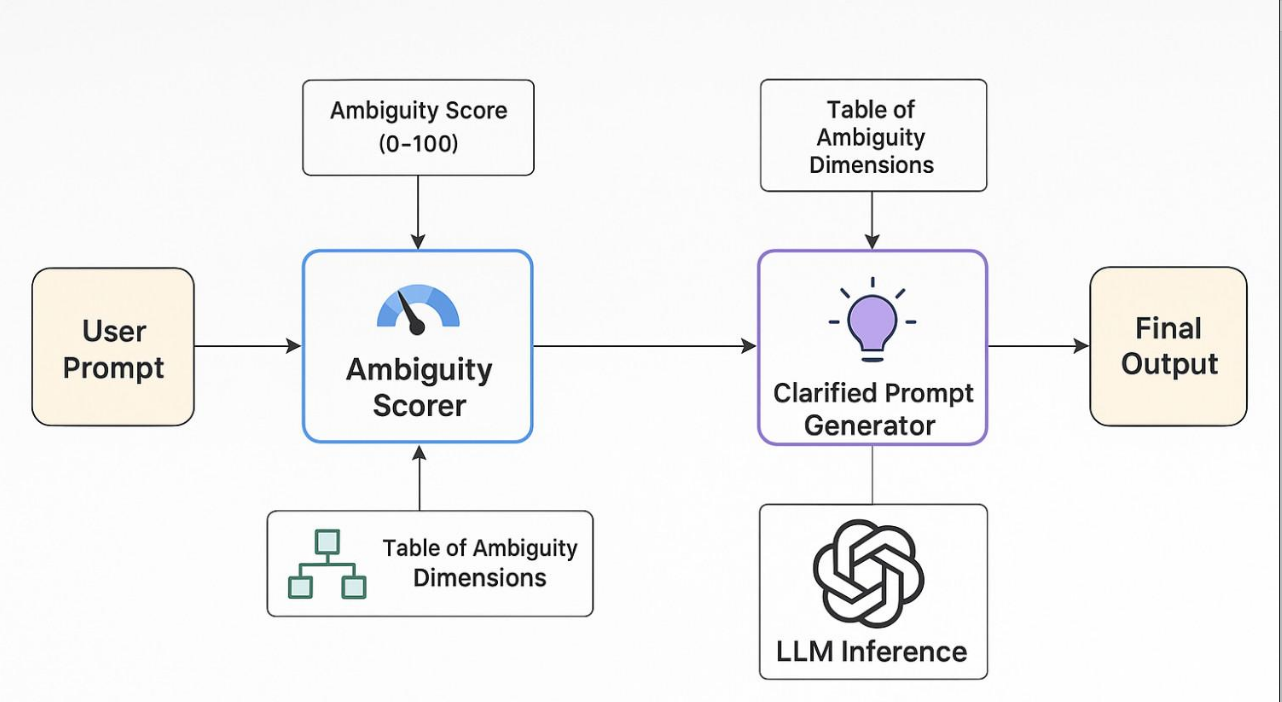
\includegraphics[width=\columnwidth]{images/Figure1.jpeg}
\caption{System Architecture.}
\label{fig_sim}
\end{figure}

\subsection{Core Implementation}

\subsubsection{Frontend Service Integration with Puter.js}
A key novelty of our approach is the use of \textbf{Puter.js}, a serverless JavaScript SDK allowing inference from a browser directly, without server-side authentication, cloud storage, and database access, as well as performing powerful LLM inference. For a developer, that opens the doorways to lots of things including multi-model AI chat, user authentication, and KeePassCloud storage—from the client-side scripting only by adding a single \texttt{<script>} tag.
\\
\\
\textbf{Advantages of Puter.js Integration:}
\begin{itemize}
    \item \textbf{True Serverless:} All prompt analysis, ambiguity scoring, clarifications, and inferencing occur in your browser—no backend to deploy or manage.
    \item \textbf{Unified API for Cloud \& AI:} Storage, user-session management, LLM calls all have similar, user-friendly APIs.
    \item \textbf{Bet on User Privacy \& Security:} Data is kept at the client; it will only be shared/stored via cloud APIs if the customer agrees.
    \item \textbf{Rapid Prototyping:} No hassle setup means you can easily create demos and scale all the way to production.
\end{itemize}

\textit{Example usage:}

\begin{lstlisting}[language=HTML]
<script src="https://js.puter.com/v2/"></script>
<script>
    puter.ai.chat("Hello AI! This is Adnan & Dr. Aiman Abu Samra.");
</script>
\end{lstlisting}

This seamless integration allows any LLM-based workflow to be executed natively in the browser and massively increases the accessibility of the technology to developers and end-users.

\subsubsection{Modular LLM Processing: `generateLLMResponses` and `analyzeLLMResponses`}
The heart of both our systems is two modular JavaScript functions:

\paragraph{`generateLLMResponses`}
Manages sending prompts to the chosen LLM (GPT-4 or otherwise), which controls model selection and API requests through Puter.js. A prompt generator is employed to express both baseline (potentially ambiguous) prompts and disambiguated prompts output by the analyzer.
\begin{itemize}
    \item It accepts user/system prompts and the model choice.
    \item Invokes the LLM API via Puter.js.
    \item It returns the raw model output to the UI.
\end{itemize}

\paragraph{`analyzeLLMResponses`}
Structured core analysis is triggered by wrapping the user prompt in a highly structured meta-prompt sent to the analysis LLM.
Within this meta-prompt, the LLM is directed to:
\begin{itemize}
    \item Assign a score reflecting the degree of uncertainty (range between 0 and 100)
    \item Record all uncertain dimensions, their labels, impact levels, as well as two (or more) relative assumptions.
    \item Create clear rewrites of the prompt.
\end{itemize}
The LLM returns tabulated results in a strict JSON schema, facilitating predictable UI rendering and post-processing tasks. The meta-prompt template we used is as follows:

\begin{lstlisting}[language=,frame=single]
Analyze the ambiguity of this prompt: "${promptText}"
                 Return in JSON:
                 - ambiguityRating (0-100)
                 - analysisTable: [ { impactLevel, dimensionName, possibleAssumptions(two assumed values)} ]
                 - suggestedClarifiedPrompt: clarified prompt assumptions for the missing parameters
\end{lstlisting}

\textbf{Typical workflow:}
\begin{enumerate}
    \item User submits a prompt.
    \item `analyzeLLMResponses` measures ambiguity and provides analysis and feedback.
    \item User chooses a refined prompt and changes it if necessary.
    \item `generateLLMResponses` fetches the LLM response for the clarified prompt.
\end{enumerate}

\subsubsection{Interactive Chat Interface}
The frontend is a feature-rich, browser-based chat interface fluent in the language of JavaScript and written in Puter.js for all AI operations.

\textbf{Key features:}
\begin{itemize}
    \item \textbf{Model Selection:} Users select from the LLMs in the supported list (default: GPT-4).
    \item \textbf{Message Processing in Real Time:} Processing messages in real time from the user and the AI, which can be copied or exported.
    \item \textbf{Multimodal Support:} It can take images uploaded or pasted by users as content for analysis, together with text prompts.
    \item \textbf{Prompt Clarification Modal:} The button “Clarify” and its three sub-checkboxes are intended to immediately trigger the detect process of ambiguities and, thus, instead of only obtaining scores and ambiguity dimensions, also obtain proposed rewrites in a modal window with a single click to insert.
    \item \textbf{Export/Copy:} The whole chat can be saved (Word supported) or copied in a formatted manner.
    \item \textbf{User Experience Improvements:} Feedback messages, auto-size inputs, superior error handling.
\end{itemize}

\textbf{Workflow:}
\begin{enumerate}
    \item User enters a prompt and/or image.
    \item The prompt is sent to the LLM through Puter.js; the AI reply is displayed.
    \item “Clarify” examines ambiguity and shows structured feedback and advice.
    \item User can export and copy chat history.
\end{enumerate}

\textit{For a live demo, see: \url{https://amuammer.github.io/ai}.}

\begin{figure}[!t]
\centering
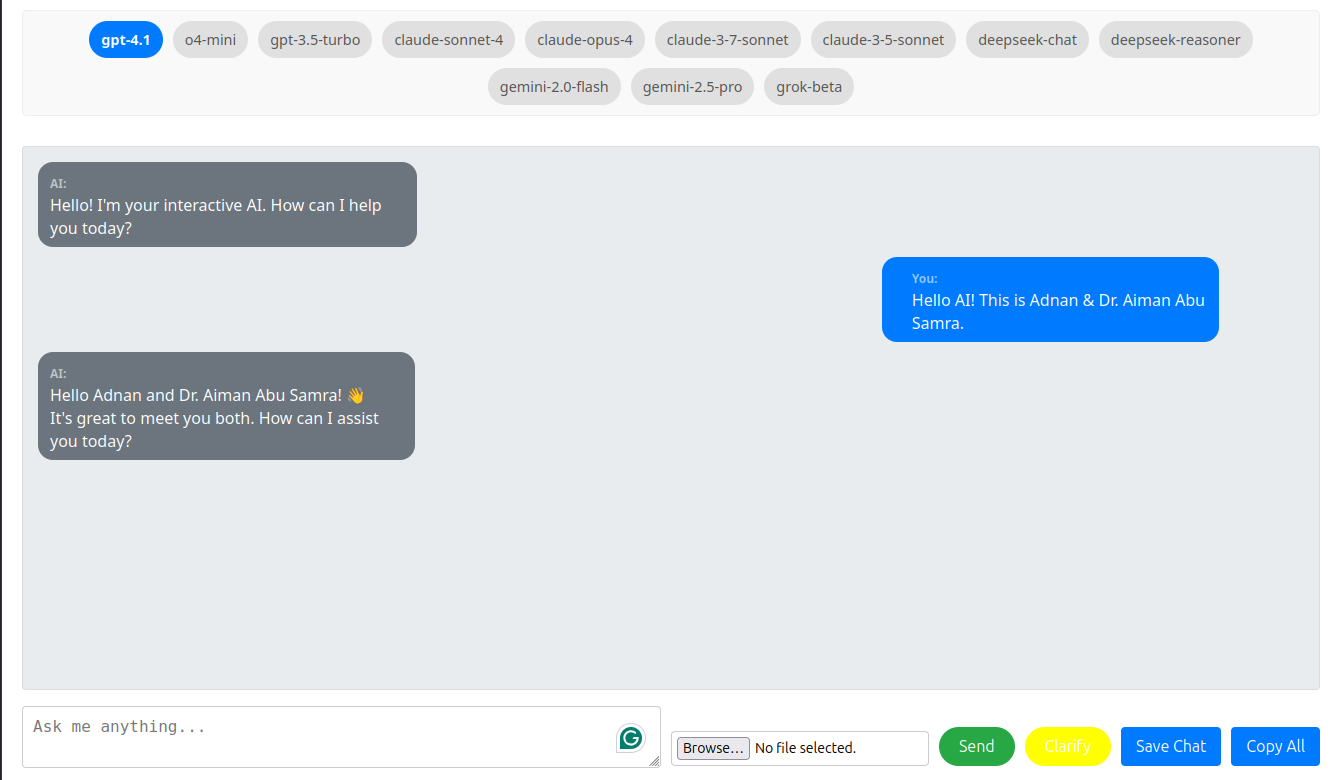
\includegraphics[width=\columnwidth]{images/Figure2.jpeg}
\caption{Chat UI.}
\label{fig_chatui}
\end{figure}


\subsection{Dataset Preparation and Processing Source Code}
In order to systematically test and compare our ambiguity analysis framework, we implemented a set of scripts to create, analyze, and combine LLM responses. All preparation and pre-processing of the datasets were conducted in fully transparent client-side and Node.js code, providing a framework that reproduces and can be extended.

\textbf{Key steps and scripts:}
\begin{itemize}
    \item \textbf{Prompt and Baseline Generation}
        \begin{itemize}
            \item \texttt{\lstinline!1.collect-generatorLLM-responses.html!}: Uses Puter.js itself in the browser to send each ambiguous prompt to the LLM and save the raw baseline response.
        \end{itemize}
    \item \textbf{Ambiguity Analysis Collection}
        \begin{itemize}
            \item \texttt{\lstinline!2.collect-analyzerLLM-responses.html!}: Uses Puter.js in the browser to serve prompts over the ambiguity analysis meta-prompt and aggregate structured analyzer responses.
        \end{itemize}
    \item \textbf{CSV Export and Deduplication}
        \begin{itemize}
            \item \texttt{\lstinline!back-queried-LLM-to-csv-ambigous.js!}: Node.js script that generates unique (field, prompt) pairs from a dataset and saves them into a CSV to be processed.
        \end{itemize}
    \item \textbf{Deduplication, Grouping, and Indexing}
        \begin{itemize}
            \item \texttt{\lstinline!ordering-dataset.js!}: Node.js script that strips duplicates, gives entries a global identifier \& sequential index in that stream, and groups entries by field for further analysis.
        \end{itemize}
    \item \textbf{Changing Generator and Analyzer Outputs}
        \begin{itemize}
            \item \texttt{\lstinline!3.mergeLLMResponses.js!}: Node.js script that combines the baseline LLM predictions with the accompanying ambiguity analyses, matching by prompt and standardizing the indexing across the dataset.
        \end{itemize}
\end{itemize}
Each script is documented and configurable for reusability with other jobs or LLMs. Output data sets are utilized in the experimental sections (refer to Section 5). Full code and reproducibility details are available at \textit{our repository\cite{amuammer2025promptframework}: \url{https://github.com/amuammer/ai}.}

\section{Experiments}
In order to validate the effectiveness of our pre-processing, an experimental protocol in terms of token-level cost analysis is developed.

\subsection{Dataset and Procedure}
We composed a benchmark set of extremely ambiguous prompts across various tasks as follows:
\begin{itemize}
    \item Business Communication (15)
    \item Code Generation (15)
    \item Data Analysis (15)
    \item Education (15)
    \item Technical Writing (15)
    \item Human Resources (15)
    \item General Question Answering (15)
\end{itemize}

\begin{figure}[!t]
\centering
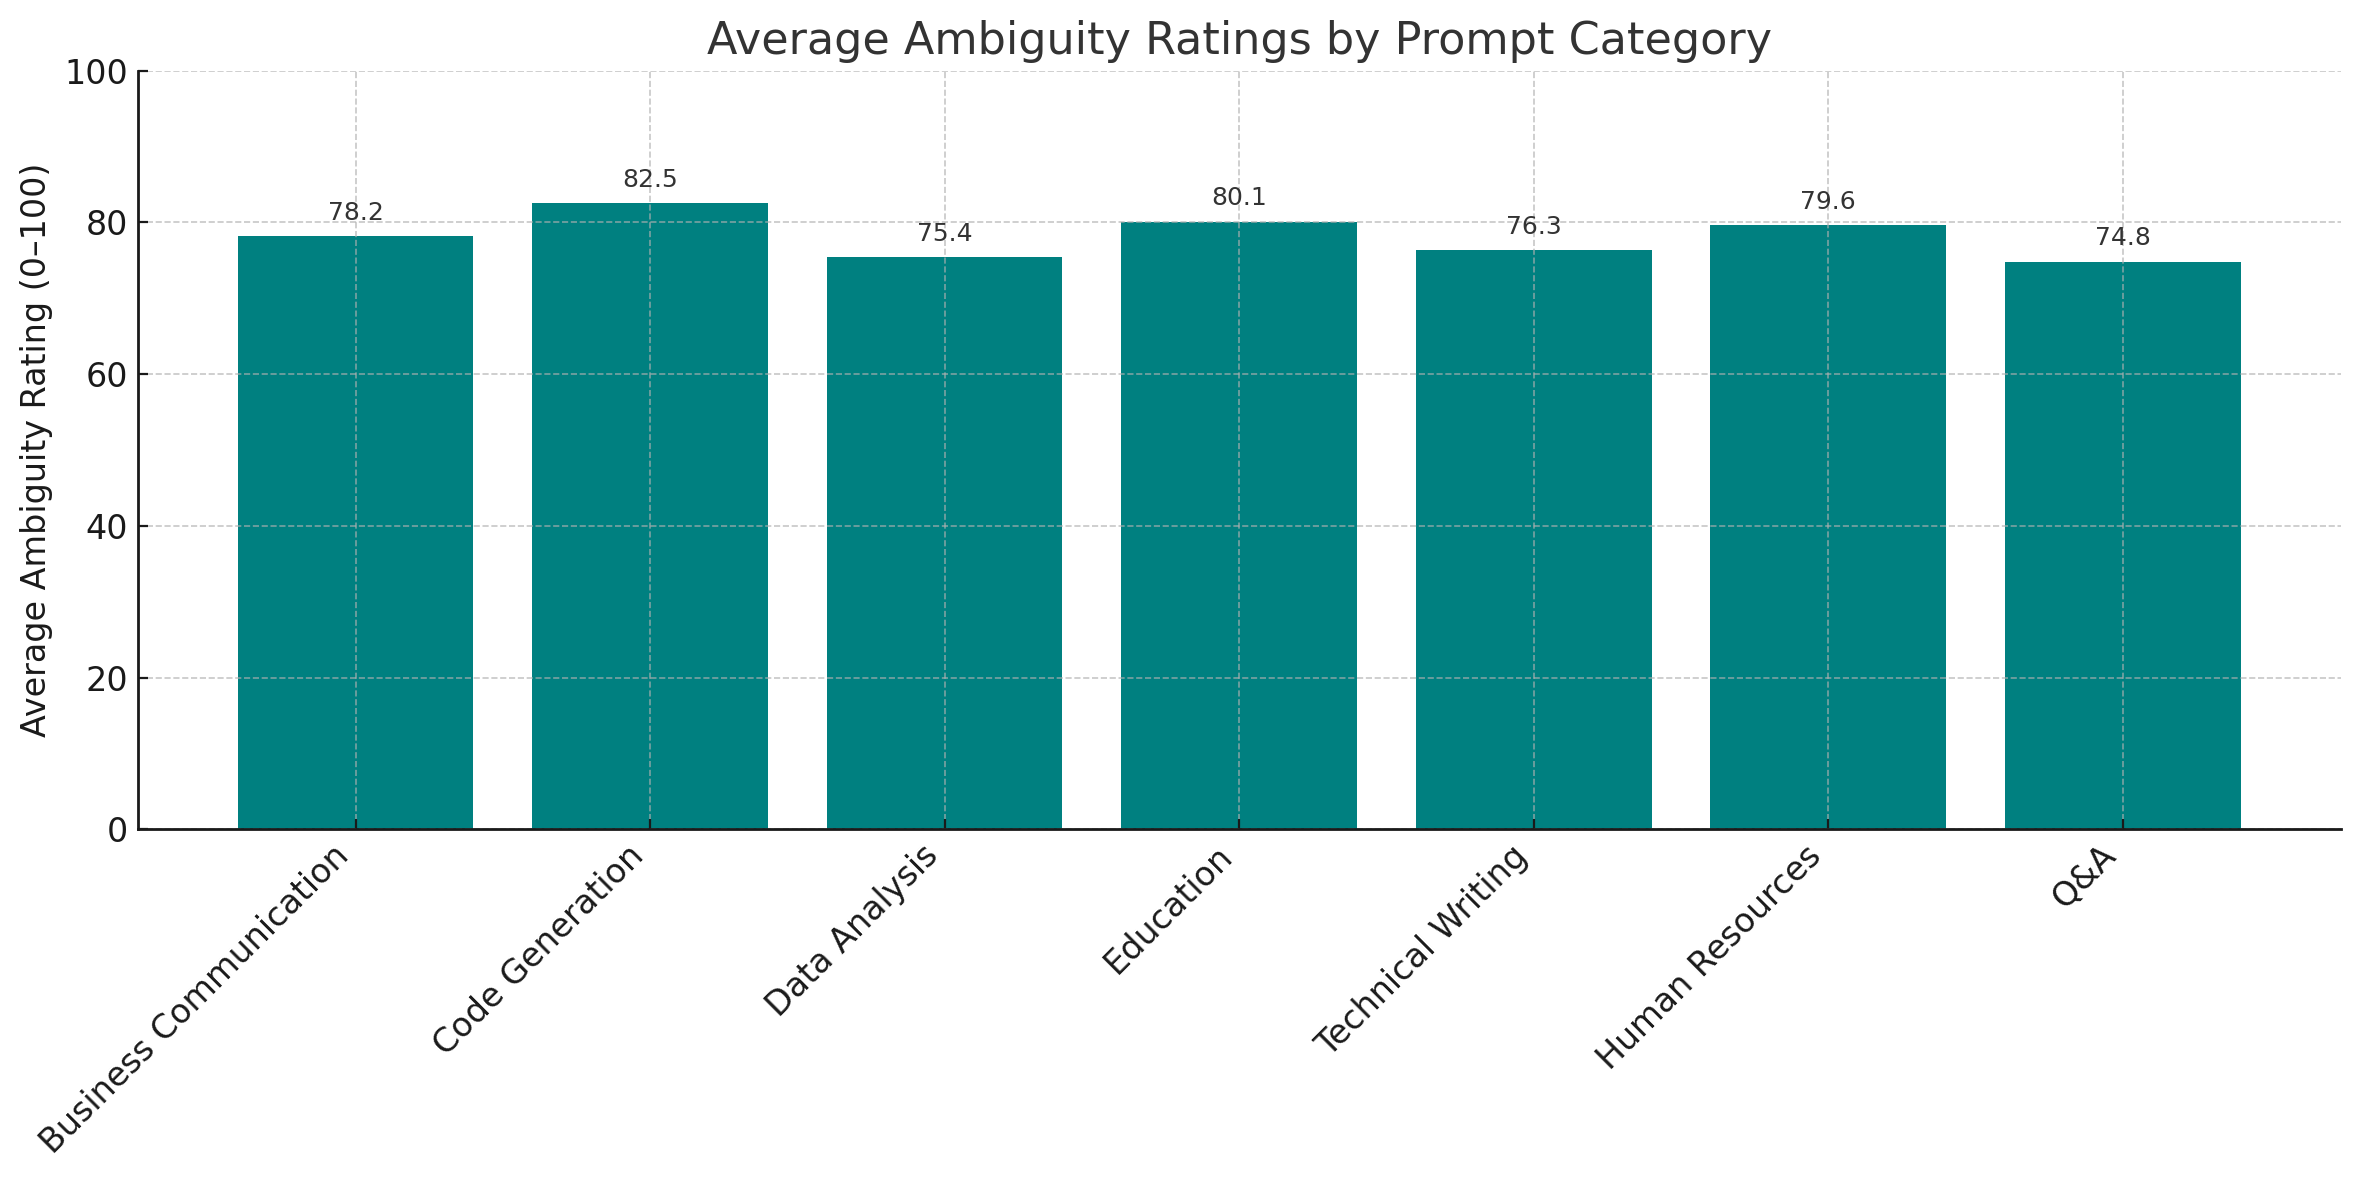
\includegraphics[width=\columnwidth]{images/Figure3.jpeg}
\caption{ambiguityRatingPerField.}
\label{fig_ratingperfield}
\end{figure}

For each ambiguous command, we performed the following:
\begin{enumerate}
    \item \textbf{Simulate a Wasted Cycle:}
    The \texttt{original\_prompt} was submitted to a generation LLM (GPT-4) to get a \texttt{baseline\_response}, and simulate the response of an initial, possibly unhelpful answer.
    \item \textbf{User Clarification:}
    A human expert authored a \texttt{followup\_prompt}—an even more explicit reformulation which, when given as input, should enable the user to provide a valid response.
    \item \textbf{System Analysis:}
    The same \texttt{original\_prompt} was processed by our model LLM, resulting in a structured \texttt{analyzer\_response} with ambiguity score, diagnosis, and suggestions for the prompt.
    \item \textbf{Token Counting:}
    For each prompt, we reported token counts for:
    \begin{itemize}
        \item \texttt{T\_original\_prompt}
        \item \texttt{T\_baseline\_response}
        \item \texttt{T\_followup\_prompt}
        \item \texttt{T\_analyzer\_response}
        \item The hard-coded token count of the \texttt{T\_analyzer\_prompt} template is (31)
    \end{itemize}
\end{enumerate}

\subsection{Evaluation Procedure}
The authors have developed an automatic script that performs the following steps for each prompt in the dataset:
\begin{enumerate}
   \item Send the \texttt{ambiguous\_prompt} to a generation LLM Model (e.g., GPT-4), and a  \texttt{baseline\_response} is returned.
    \item Pass \texttt{ambiguous\_prompt} to the Analysis LLM Model and get \texttt{ambiguityRating}, \texttt{analysisTable}, and \texttt{suggestedClarifiedPrompt}.
    \item Transfer the \texttt{suggestedClarifiedPrompt} again to the generation LLM Model, and a \texttt{clarified\_response} is generated in return.
\end{enumerate}

\subsection{Quantifying Reduction in Computation Waste and ROI}
We introduce a token-driven cost-benefit model to evaluate the effectiveness of our system.

\textbf{Cost Metrics:}
\begin{enumerate}
    \item \textbf{Computational Cost Savings:}
    \begin{itemize}
        \item \textbf{Cost of Preventive Analysis (\(C_{\text{analysis}}\)):}
            The complexity of finding an ambiguity includes:
        \begin{itemize}
            \item Tokens used in the analyzer meta-prompt template (\(T_{\text{analyzer\_prompt}}\))
            \item Tokens for the original user prompt (\(T_{\text{original\_prompt}}\))
            \item Tokens in the response from the analyzer (\(T_{\text{analyzer\_response}}\))
        \end{itemize}
        \begin{align}
        C_{\text{analysis}} &= T_{\text{analyzer\_prompt}} 
          + T_{\text{original\_prompt}} \notag \\
        &\quad + T_{\text{analyzer\_response}}
        \end{align}
        
        \item \textbf{Cost of a Wasted Generation Cycle (\(C_{\text{wasted}}\)):}
        The penalty of a failed transaction due to ambiguity, where:
        \begin{itemize}
            \item Tokens in the source prompt
            \item Tokens in the non-effective baseline response
            \item Tokens in user follow-up clarification
        \end{itemize}
        \begin{align}
        C_{\text{wasted}} &= T_{\text{original\_prompt}} 
          + T_{\text{baseline\_response}} \notag \\
        &\quad + T_{\text{followup\_prompt}}
        \end{align}
        
        \item \textbf{Computational Cost Savings Metric:}
        Mean of the difference between \(C_{\text{wasted}}\) and \(C_{\text{analysis}}\), for all prompts.
    \end{itemize}
        \begin{equation}
        \begin{aligned}
        \text{Saving in Computational Cost} \\
        = C_{\text{wasted}} - C_{\text{analysis}}
        \end{aligned}
        \end{equation}
    
    \item \textbf{Time-to-Satisfactory-Response:}
    \begin{itemize}
        \item \textbf{Definition:}
        The time taken from the ambiguous prompt to the first useful LLM response.
        \item \textbf{Measurement:}
        For each message, we log the time, in the baseline (no analyzer was intervening) and in the presence of the analyzer using the system design where the S indicates the encounters where a satisfactory message is found both with and without help from the analyzer.
        \item \textbf{Time Reduction Metric:}
        The average decrease in time-to-satisfactory-response attributable to the analyzer system.  
    \end{itemize}
\end{enumerate}

\subsection{Decision Criterion}
Our system yields a net computational and temporal benefit whenever:
\begin{equation}
C_{\text{analysis}} < C_{\text{wasted}}
\end{equation}
and
\begin{equation}
C_{\text{char}_{\text{analyzer}}} < C_{\text{char}_{\text{baseline}}}
\end{equation}

\section{Assessment: Analysis of Computational Cost-Benefit and Time Efficiency}
We measured the ROI of these macros by comparing the token cost and time cost of a forward analysis with the cost of failing an interaction cycle.

\subsection{Defining Metrics}
\begin{table}[t]
\begin{center}
\small  % Add this for more compact tables
\begin{tabular}{p{3.3cm}p{0.7cm}p{3.7cm}}
\hline \bf Metric & \bf Type & \bf Description \\ \hline
Ambiguity Score Accuracy & Quant. & Alignment with human labels \\
Dimension Coverage & Quant. & distinct ambiguity types detected \\
Clarification Success Rate & Quant. & clarifications resolving ambiguity \\
LLM Output Quality & Qual. & Human/automated rating of response \\
Token Cost Savings & Quant. & \( C_{\text{wasted}} - C_{\text{analysis}} \) \\
Time-to-Resolution & Quant. & Latency from prompt to correct answer \\
User Satisfaction & Qual. & User surveys, ratings \\
Adoption Rate & Quant. & Users accepting clarified prompts \\
Failure Rate & Quant. & System robustness, error rate \\ \bottomrule
\end{tabular}
\end{center}
\caption{\label{tab:metrics} Evaluation Metrics}
\end{table}


The metrics above are all things we could go with, but we select:
\begin{itemize}
    \item \textbf{Computational Cost Savings:}
    The trivial saving in tokens associated with the application of the analyzer system as stated above.
    \item \textbf{Time-to-Satisfactory-Response:}
    The amount of time saved between submitting the prompt and receiving an acceptable answer via the analyzer.
\end{itemize}

\subsection{Results}
Over the complete set of prompts in the benchmark, the average costs were:
\begin{verbatim}
  c_wasted sum = 28,956
  c_analysis sum = 14,641
  Total entries = 105
  avg_char_baseline = 1241.5 char
  avg_char_analyzer = 179 char
\end{verbatim}

\begin{table}[H]
\begin{center}
\small  % Add this for more compact tables
\begin{tabular}{p{5.4cm}p{1.8cm}}
\hline \bf {Metric} & \bf {Avg Value} \\ \hline
\textbf{Avg. C\_wasted (Failure, tokens)} & 275.8 tokens \\
\textbf{Avg. C\_analysis (Prevention, tokens)} & 139.4 tokens \\
\textbf{Net Computational Savings per Prompt}  & 136.4 tokens \\
\textbf{Avg. Reading Baseline Response (Failure)} & 82.77 sec \\
\textbf{Avg. Reading Analyzer Response}  & 11.93 sec  \\
\textbf{Net Time Saved in Reading Effort} & 70.83 sec  \\ \bottomrule
\end{tabular}
\end{center}
\caption{\label{tab:results} Average Cost and Time Savings}
\end{table}

\begin{figure}[!t]
\centering
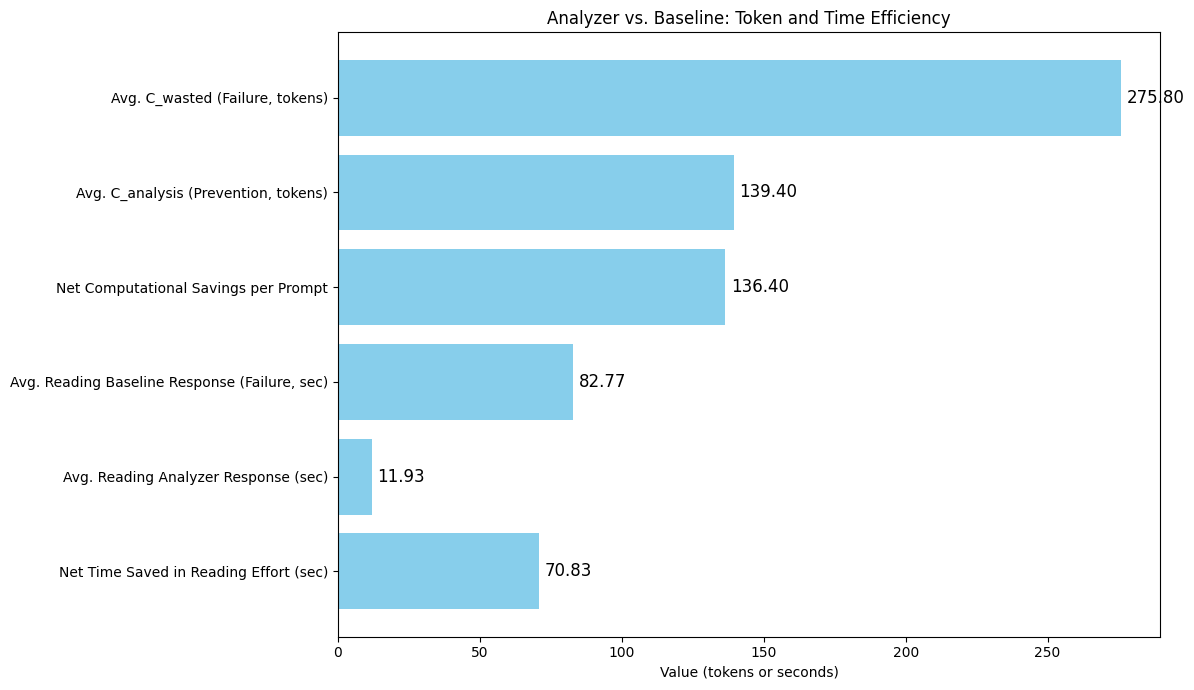
\includegraphics[width=\columnwidth]{images/Figure4.jpeg}
\caption{tokenAndTimeEffieciency.}
\label{fig_efficiency}
\end{figure}

The reward of engaging the analyzer LLM is, on average, half the token cost of an unsuccessful interaction. Preventative analysis using 139.4 tokens prevents 275.8 tokens of waste on average for each ambiguous prompt—a 49.5\% reduction in computational cost per interaction. The analyzer eliminates much of the original thinking and typing time of writing a follow-up. But it does not remove user effort entirely—it offloads some of that effort to creating an edit clarification.

\texttt{Without Analyzer: User Prompt -> User reads reply → recognizes failure → writes up follow-up prompt → hits send}

\texttt{With Analyzer: User Prompt -> Special malware protect → Analyzer creates cleaned prompt User reviews/edits -> click sends}

\textbf{Reading Speed Assumptions (According on Research)}
Average adult reading speed:
200–250 words per minute
1000–1250 characters per minute (assuming ~5 characters per word)

So:
\texttt{1000 characters / 60 seconds = ~16.7 characters per second}

\textbf{Let's presume a modest speed of reading:}
\texttt{15 characters per second}

\textbf{Average total baseline response characters to find ambiguity = ~1241.5 char and analyzer response = ~179 char}

When analyzing failures, the users spend on average around 83 seconds reading the ambiguous baseline responses, while around 12 seconds for the structured analyzer outputs. This results in a 71\% reduction in reading time, the potential for increased comprehension, as well as a decrease in cognitive load during the disambiguation process.

\begin{figure}[!t]
\centering
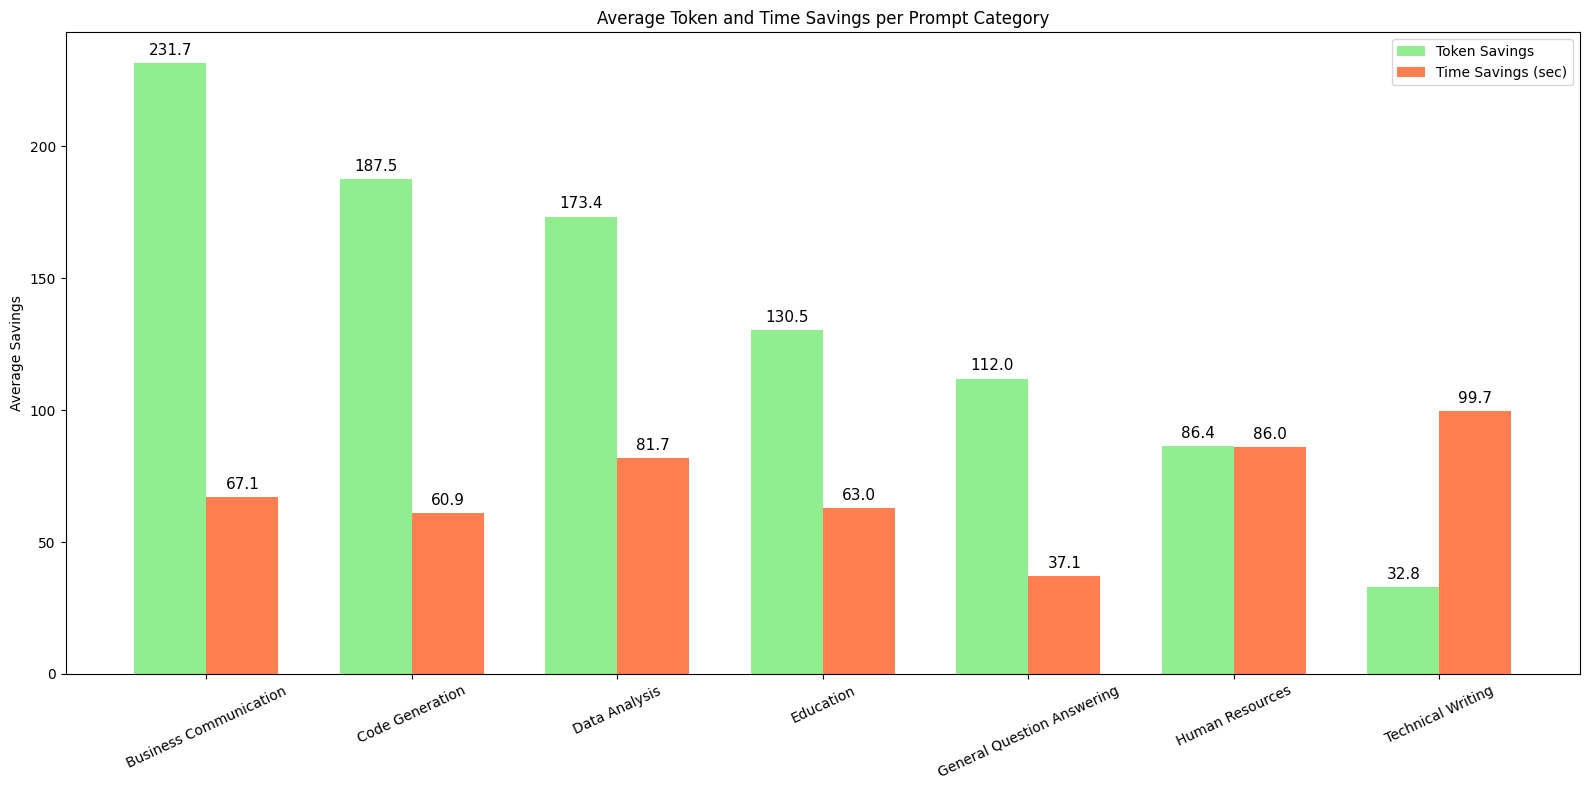
\includegraphics[width=\columnwidth]{images/Figure5.jpeg}
\caption{tokeAndTimePerField.}
\label{fig_timeperfield}
\end{figure}

\section{Discussion and Future Work}
Our results demonstrate that ambiguity analysis integration is beneficial in both computational and practical aspects when applied to LLM pipelines:
\begin{itemize}
    \item High requests resolution ambiguity requires preprocessing a fast and cost-efficient method that minimizes trial and error for the user after solving.
    \item The approach is scalable where there are metered/limited LLMs (e.g., API services).
\end{itemize}

\textbf{Future Directions:}
\begin{itemize}
    \item Adaptive model design allowing for localization of the probability of ambiguity prior to analysis start-up.
    \item Measure the non-computational benefits like user satisfaction and task success.
    \item Broadening the application domain to multi-turn dialogues where ambiguity problems may accumulate.
\end{itemize}

\section{Conclusion}

In particular, our system can automatically score how ambiguous a prompt is and identify and generate clarified versions of prompts, thereby significantly reducing the waste of computation in LLM-based pipelines.

\section*{Acknowledgment}
The authors thank the open-source community and contributors to the \texttt{amuammer/ai} project for inspiration and support.


%\bibliography{references}
%\bibliographystyle{tacl2018v2}

\bibliography{references}
\bibliographystyle{acl_natbib}


\end{document}